\section{Análise de Variância (ANOVA)}

	``A ANOVA é empregada para verificar se há diferença sistemática entre as médias de resultados \textbf{normalmente distribuídos} de experimentos randômicos.
	
	Trata-se de um método estatístico, que por meio de
\textbf{teste de igualdade de médias}, verifica se fatores (variáveis independentes) produzem mudanças sistemáticas em alguma variável de interesse (variável dependente).

	Os fatores propostos podem ser variáveis quantitativas
ou qualitativas, enquanto a variável dependente deve ser quantitativa.

	Todos os sujeitos (participantes ou unidades experimentais) de determinado grupo recebem o mesmo tratamento, assegurando que as diferenças sistemáticas entre médias de grupos possam ser atribuídas aos efeitos dos diferentes tratamentos" \cite{torres} .

	\subsection{Pressupostos da ANOVA \cite{torres}}

			\subsubsection{As observações dentro de cada grupo têm distribuição normal}
			
				``A normalidade não é restritiva ao uso da ANOVA quando o número de elementos em cada grupo é relativamente elevado $(n \geq 30)$ ;

				A não normalidade tem consequências mínimas na interpretação dos resultados, a não ser que a distribuição seja muito viesada".

				\textbf{Outras Observações}

					A normalidade é função da combinação de 2 medidas: assimetria e curtose. Se ela é normal ela é simétrica e meso-cúrtica;

					Caso ela não dê normal, uma possibildiade é calcular assimetria e a curtose. Então se divide as duas pelo desvio padrão;

					Se for normal, a divisão da assimetria/desvio padrão e curtose/desvio padrão deve ficar entre $ (-1,96 ; 1,96) $.

			\subsubsection{As observações são independentes entre si}
				Se as observações foram coletadas de maneira independente, logo os tratamentos serão independentes entre si (e.g. grupo experimental x grupo de controle).			
			
			\subsubsection{As variâncias de cada grupo são iguais entre si, \\ ou seja, há homocedasticidade}
			
				``O teste F é robusto a violações de homocedasticidade quando o número de observações em cada grupo é igual ou aproximadamente igual (considera-se grupos de dimensões semelhantes quando o quociente entre a maior dimensão e a menor for inferior a 1,5 - \textbf{se a razão entre a amostra de tamanho maior dividido pela amostra de tamanho menor der até 1,5 = OK});

				Quando os $ n $ não são iguais ou semelhantes e há grande afastamento tanto da normalidade como da homocedasticidade, põe-se em risco as conclusões tidas na análise de variância. Nesta situação recomenda-se utilizar testes alternativos não paramétricos de Kruskal-Wallis".

	\subsection{Cálculo da ANOVA}

		\subsubsection{Quadro da ANOVA}

			\begin{table}[H]

				\centering
		
				\begin{tabularx}{\textwidth}{X <{\centering} X <{\centering} X <{\centering} X <{\centering} X <{\centering}}
			
					Fonte de & Soma dos & Grau de & Quadrados & \multirow{2}{*}{Teste F} \\
				Variação & Quadrados & Liberdade & Médios \\
				
					\noalign{\smallskip} \hline \noalign{\smallskip}
				
					Entre & \multirow{2}{*}{$ Q_{e} $} & \multirow{2}{*}{$ k -1 $} & \multirow{2}{*}{$ S^{2}_{e} = \cfrac{Q_{e}}{k - 1} $} & \multirow{7}{*}{$ F_{\text{cal}} = \cfrac{S^{2}_{e}}{S^{2}_{r}} $} \\
					Tratamentos & & & & \\
				
					\noalign{\smallskip} \cline{1-4} \noalign{\smallskip}
				
					Dentro das & \multirow{3}{*}{$ Q_{r} = Q_{t} - Q_{e} $} & \multirow{3}{*}{$ n - k $} & \multirow{3}{*}{$ S^{2}_{r} = \cfrac{Q_{t} - Q_{e}}{n - k} $} & \\
					Amostras & & & & \\
					(Residual) & & & & \\
				
					\noalign{\smallskip} \cline{1-4} \noalign{\smallskip}
				
					Total & $ Q_{t} $ & $ n - 1 $ & &
				
				\end{tabularx}

			\end{table}

		\subsubsection{Fórmulas}
	
			\paragraph{Soma dos Quadrados Totais}
		
				{\Large $ Q_{t} = \sum \limits^{k}_{i=1} \sum \limits^{n_{i}}_{j=1} x^{2}_{ij} - C$}
			
			\paragraph{Soma dos Quadrados Entre Tratamentos}
		
				{\Large $ Q_{e} = \sum \limits_{i} \begin{bmatrix} \cfrac{ \begin{pmatrix} \sum \limits_{j} x_{ij} \end{pmatrix}^{2}}{n_{i}} \ \ \end{bmatrix} - C$}
			
			\paragraph{Constante}
		
				{\Large $ C = \cfrac{\begin{pmatrix} \sum \limits^{k}_{i=1} \sum \limits^{n_{i}}_{j=1} x_{ij} \end{pmatrix}^{2}}{n} $ }
			
		\subsubsection{Tabela de Contingência \cite{bussab}}
	
			\begin{table}[H]
				\centering
		
				\begin{tabularx}{\textwidth}{X <{\centering} X <{\centering} X <{\centering} X <{\centering} X <{\centering} X <{\centering} X <{\centering}}
			
					\multirow{2}{*}{Indivíduo} & \multicolumn{6}{>{\hsize=6\hsize\centering}X}{Variável} \tabularnewline
				& $ X_{1} $ & $ X_{2} $ & \dots & $ X_{j} $ & \dots & $ X_{p} $ \tabularnewline
				
					\noalign{\smallskip} \hline \noalign{\smallskip}
				
					1 & $ X_{11} $ & $ X_{12} $ & \dots & $ X_{1j} $ & \dots & $ X_{1p} $ \tabularnewline
				
					\noalign{\smallskip} \hline \noalign{\smallskip}
				
					2 & $ X_{21} $ & $ X_{22} $ & \dots & $ X_{2j} $ & \dots & $ X_{2p} $ \tabularnewline
				
					\noalign{\smallskip} \hline \noalign{\smallskip}
				
					. & . & . &  & . &  & . \tabularnewline
					. & . & . &  & . &  & . \tabularnewline
					. & . & . &  & . &  & . \tabularnewline

					\noalign{\smallskip} \hline \noalign{\smallskip}
				
					i & $ X_{i1} $ & $ X_{i2} $ & \dots & $ X_{ij} $ & \dots & $ X_{ip} $ \tabularnewline
				
					\noalign{\smallskip} \hline \noalign{\smallskip}
				
					. & . & . &  & . &  & . \tabularnewline
					. & . & . &  & . &  & . \tabularnewline
					. & . & . &  & . &  & . \tabularnewline
				
					\noalign{\smallskip} \hline \noalign{\smallskip}
				
					n & $ X_{n1} $ & $ X_{n2} $ & \dots & $ X_{nj} $ & \dots & $ X_{np} $ \tabularnewline
				
				\end{tabularx}

			\end{table}
		
		\subsubsection{Utilizando a Distribuição F (Fisher–Snedecor) para Testar a Nulidade dos Estimadores}
	
			``A distribuição “F” é apropriada para a \textbf{razão das variâncias de duas amostras}, tomadas independentemente da mesma população normalmente distribuída.

			A estatística usada para testar a hipótese nula de que não existe diferença entre as variâncias é " \cite{torres}:
		
			{\Large $ F_{v_{1},v{2}} = \cfrac{S^{2}_{1}}{S^{2}_{2}} \ , \ \text{onde} \ F_{v_{1},v{2}, \text{inferior}} = \cfrac{1}{F_{v_{2},v{1}, \text{superior}}} $}
		
			\paragraph{Teste de Hipóteses}

				$
					\begin{cases}
			        \mathsf{H}_{0} : & \mu_{A} = \mu_{B} = \mu_{C} \\
			        \mathsf{H}_{a} : & \text{As médias de pelo menos dois grupos são diferentes}
			        \end{cases}
				$
		
			\paragraph{Ponto crítico}
		
				$ F_{c} \ \alpha - 1 \ ; \ k - 1 \ ; \ n - k = ?  $
		
			\paragraph{Distribuições F \cite{google}} \hspace{0cm}
		
				\begin{figure}[H]
					\centering			
					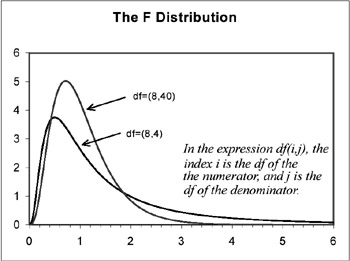
\includegraphics[height=6cm]{images/anova_distribuicao-f}
				\end{figure}					
					
	\subsection{ANOVA 1 Fator no SPSS \cite{torres}}

		Para executar a ANOVA no SPSS vá em ``Analisar $>$ Comparar Médias $>$ Análise de Variância Unidirecional...", porém não esqueça de verificar a normalidade dentro de cada grupo.

		Para verificar a normalidade utilizando o SPSS, faça os testes de Kolmogorov-Smirnov (\textbf{K-S}) e \textbf{Shapiro-Wilks} (verifique as hipóteses desses testes na seção de Regressão Linear).

		\subsubsection{Teste de Levene}

			O teste de Levene serve para verificar a homocedasticidade dentre os grupos, ou seja, se as variâncias de cada grupo são iguais entre si. ``Ele é tão sensível à violações de normalidade como o Teste de Bartlett. Porém, quando os “n” são iguais em cada grupo, a ANOVA é robusta às violações da homocedasticidade e o Teste de Levene se torna pouco útil" \cite{torres}.

			Caso não haja homocedasticidade, olhe o tamanho das amostras. Se elas não forem de tamanhos iguais ou semelhantes, não há teste paramétrico alternativo para utilizar.

			\bigskip

			\textbf{Teste de Hipóteses}

					\bigskip

					$
					\begin{cases}
						\mathsf{H}_{0} : & \text{As variâncias dentro dos grupos são homogêneas} \\
						\mathsf{H}_{a} : & \text{As variâncias dentro dos grupos não são homogêneas}
					\end{cases}
					$
			
			\bigskip \bigskip
			
			\textbf{Tabela}
			
				\begin{figure}[H]
					\centering			
					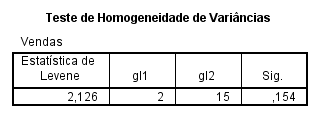
\includegraphics[height=3.5cm]{images/anova_levene}
				\end{figure}
				
		\subsubsection{Teste de Tukey}

			O teste de Tukey é um dos testes de comparação de médias mais utilizados por ser bastante rigoroso. Ele não permite comparar grupos entre si e é utilizado para testar toda e qualquer diferença entre duas médias de tratamento. É aplicado quando o teste $ F $ para tratamentos (1, 2, 3, ...) da ANOVA é significativo.

			\bigskip
			
			\textbf{Tabela}	

				\begin{figure}[H]
					\centering			
					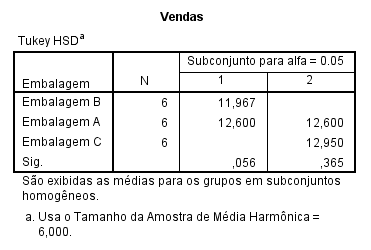
\includegraphics[height=7cm]{images/anova_tukey}
				\end{figure}

				O teste separa as médias dos grupos em subconjuntos. Quando dois ou mais grupos se encontram no mesmo subconjunto isso mostra que suas médias são iguais - a partir do nível de significância ($ \alpha $) aplicado.

				Neste caso, as embalagens A e B são iguais, assim como A e C, mas as embalagens B e C são diferentes, pois elas não aparecem juntas em nenhum subconjunto.

				A depender do que está sendo analisado, escolhe-se o tratamento ($ k $) que se destaca mais (não é igual aos outros) e que melhor se aplica à investigação (neste caso a embalagem C, pois sua média de vendas é maior do que A).
				
		\subsubsection{Tabela de Comparações Múltiplas}

			A tabela de comparações múltiplas compara as médias de diferentes tratamentos. Os testes seguem as seguintes hipóteses:

			\bigskip

			$
			\begin{cases}
				\mathsf{H}_{0} : & \mu_{1} = \mu_{2} \\
				\mathsf{H}_{a} : & \mu_{1} \neq \mu_{2}
			\end{cases} \hspace{1cm}			
			\begin{cases}
				\mathsf{H}_{0} : & \mu_{1} = \mu_{3} \\
				\mathsf{H}_{a} : & \mu_{1} \neq \mu_{3}
			\end{cases} \hspace{1cm}
			\begin{cases}
				\mathsf{H}_{0} : & \mu_{2} = \mu_{1} \\
				\mathsf{H}_{a} : & \mu_{2} \neq \mu_{1}
			\end{cases} \hspace{1cm}
			\begin{cases}
				\mathsf{H}_{0} : & \mu_{2} = \mu_{3} \\
				\mathsf{H}_{a} : & \mu_{2} \neq \mu_{3}
			\end{cases}
			$
			
			\bigskip

			E por ae vai, comparando todos os tratamentos entre si.

			\bigskip
			
			\textbf{Tabela}
			
			\begin{figure}[H]
				\centering		
				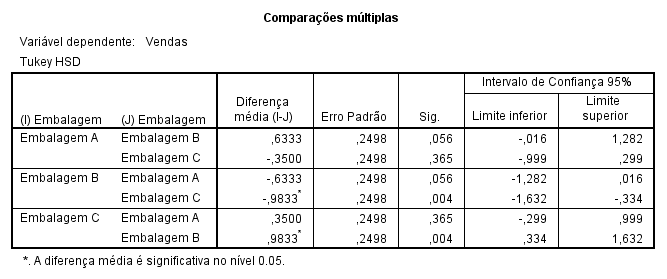
\includegraphics[height=7cm]{images/anova_comparacoes-multiplas}
			\end{figure}
			
			Neste caso podemos verificar que as médias de B e C são diferentes entre si, pois a significância é menor que 5\% ($ \alpha < 0.05$).

		\subsubsection{Tabela ANOVA}

			A tabela ANOVA comparada as médias dos grupos estudados, conforme já descrito mais acima. As hipóteses utilizadas são:

			\bigskip

			$
			\begin{cases}
				\mathsf{H}_{0} : & \mu_{1} = \mu_{2} = \mu_{3} \\
				\mathsf{H}_{a} : & \text{as médias de pelo menos dois grupos são diferentes}
			\end{cases}
			$
			
			\bigskip

			Ela pode analisar dois ou mais tratamentos. A lógica é sempre a mesma.

			\bigskip
			
			\textbf{Tabela}
			
			\begin{figure}[H]
				\centering
				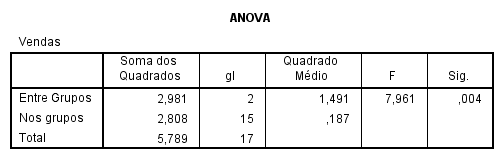
\includegraphics[height=4.5cm]{images/anova_tabela}
			\end{figure}						
			
			Neste caso rejeitamos a hipótese nula, pois a significância é menor que 5\% ($ \alpha < 0.05$).

	\subsection{ANOVA 2 Fatores \cite{torres}}

		``Sendo uma extensão da ANOVA, a ANOVA dois fatores permite analisar modelos de efeitos fixos ou mistos, analisar as tendências dos dados, proceder comparações múltiplas, analisar o efeitos das variáveis e controlar variáveis externas (fatores de segmentação da amostra)".
		É necessário primeiro fazer a ANOVA 1 fator para cada fator e seus tratamentos, antes de fazer uma ANOVA de 2 (ou mais) fatores, para verificar se os pressupostos da ANOVA estão satisfeitos.

		\bigskip

		\textbf{Teste de Hipóteses}

			\bigskip

			$
				\begin{cases}
					\mathsf{H}_{0} : & \text{não existe interação entre os fatores} \\
					\mathsf{H}_{a} : & \text{existe interação entre os fatores}
				\end{cases}
			$

	\subsection{ANOVA 2 Fatores no SPSS \cite{torres}}

		Para realizar a ANOVA 2 fatores no SPSS vá em Analisar $>$ Modelo linear geral $>$ Univariado.

		\subsubsection{Passo a Passo}

			\begin{figure}[H]
			
				\centering
				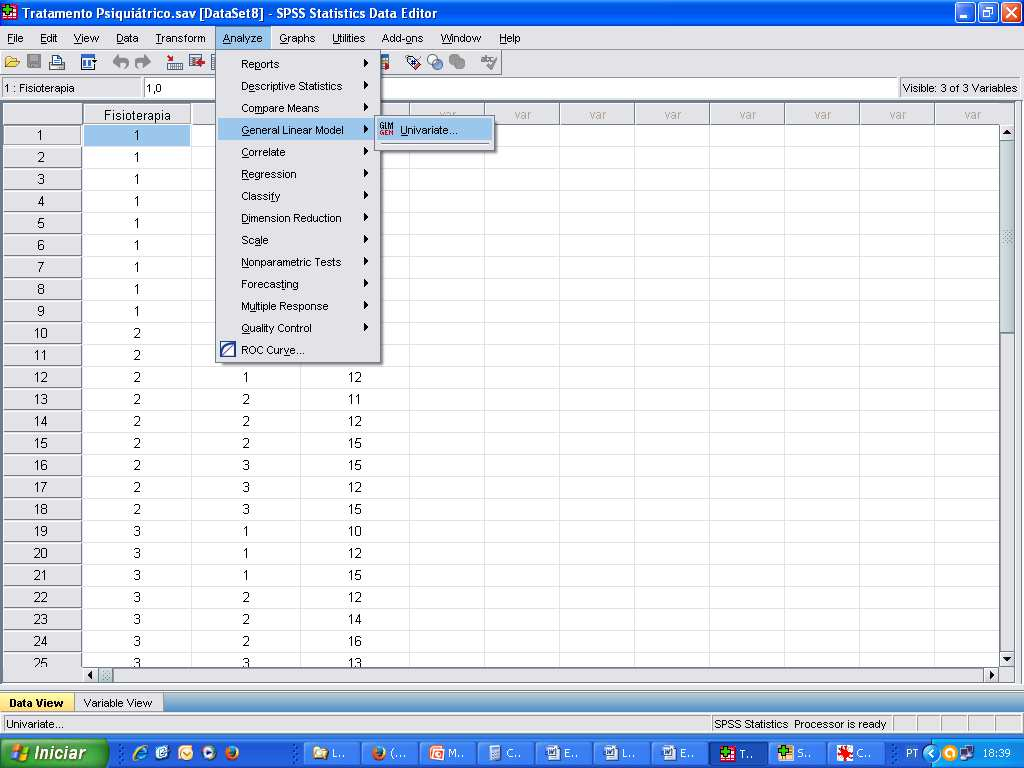
\includegraphics[height=8cm]{images/anova2_passo-a-passo_1}
			\end{figure}			
			
			\begin{figure}[H]
			
				\centering
				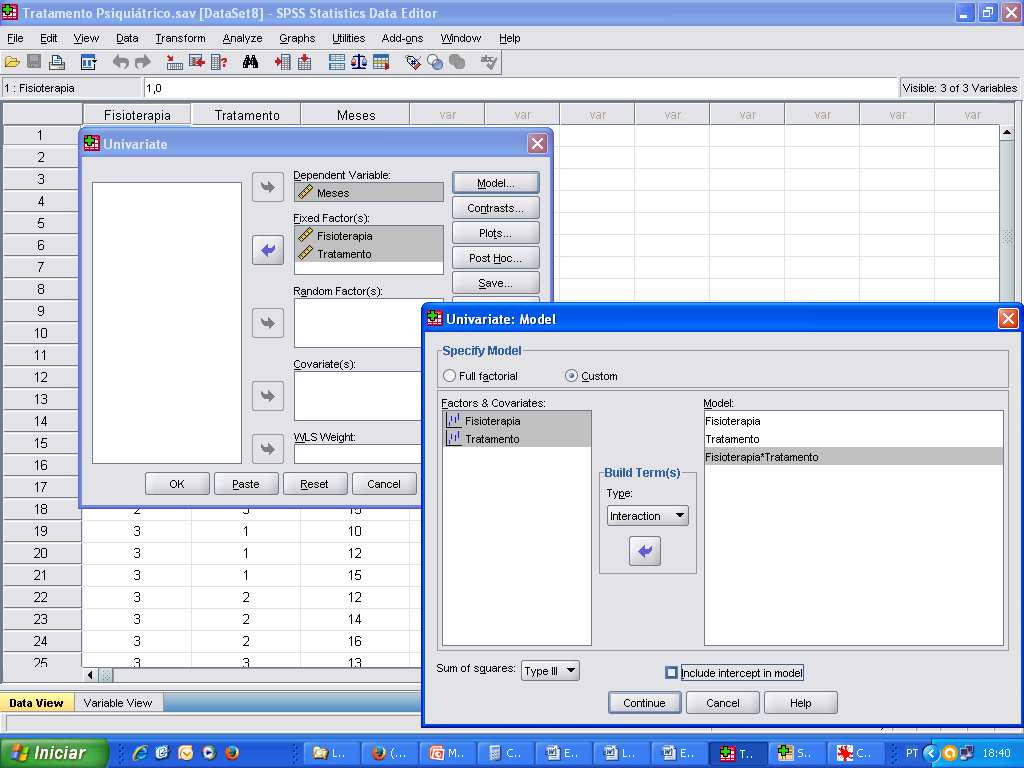
\includegraphics[height=8cm]{images/anova2_passo-a-passo_2}
			\end{figure}
			
			\begin{figure}[H]
			
				\centering
				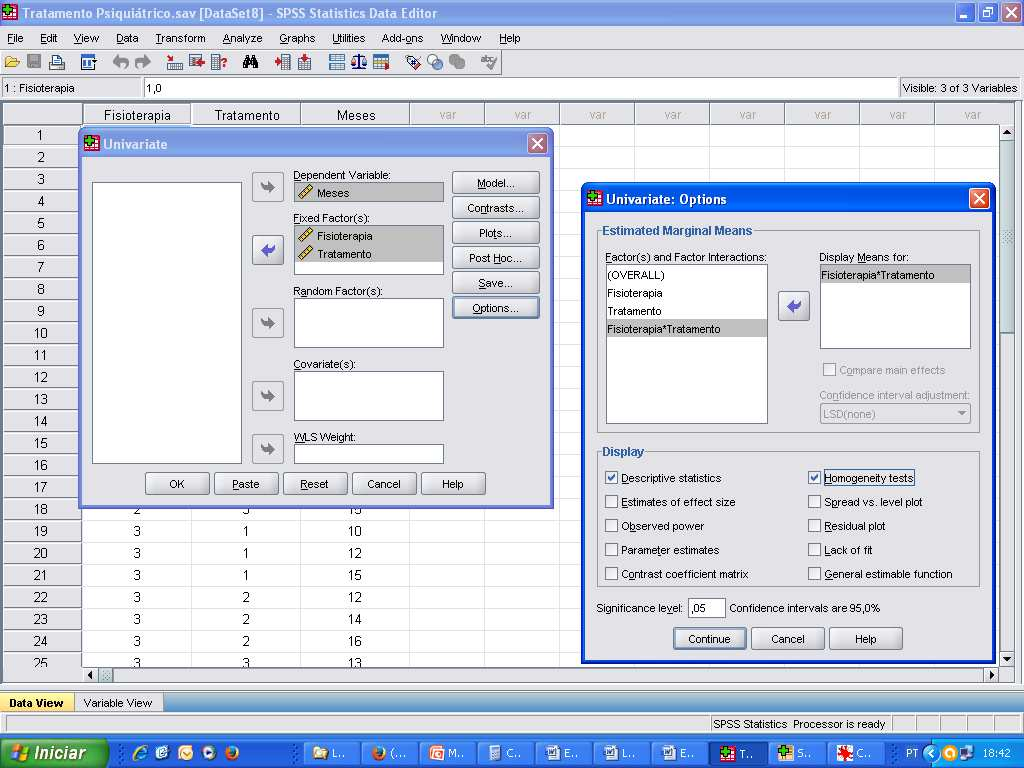
\includegraphics[height=8cm]{images/anova2_passo-a-passo_3}
			\end{figure}
		\subsubsection{Análise}

			Primeiro verifique a homocedasticidade dente os fatores pelo teste de Levene.

			O teste de hipótese da ANOVA 2 fatores se encontra na tabela de "Testes de efeitos entre sujeitos". O que nos importa aqui é a interação entre os fatores ("Fator 1*Fator 2"), logo, verifique a significância da interação pelas hipóteses da ANOVA 2 fatores.